% !TeX root = ../../main.tex
% Add the above to each chapter to make compiling the PDF easier in some editors.

\chapter{Introduction}\label{chapter:introduction}
Reinforcement learning \textbf{(RL)} is an area of machine learning inspired by behaviorist psychology, which has revolutionized our understanding of learning in the brain in the last 20 years. Unlike other machine learning approaches, that are dependent on \textit{pre-collected data}, Reinforcement Learning is a type of semi-supervised machine learning approach that which allows an agent to take actions and interact with an environment so as to maximize the total rewards.

Reinforcement learning is the closest field to Artificial General Intelligence, which mimic the human’s ability to learn from its experiences. It is best applied to situations where algorithms have to take a decision according to their environment.

Artificial General Intelligence \textbf{(AGI)} is one such concept where a machine is able to successfully perform any intellectual task that a human being can. AGI has been the most sought-after goal in the entire field of computer science. Most of the current AI applications are problems specific, and they barely touch down to the hopes of AGI. But, with reinforcement learning, achieving the goal of AGI is quite a possibility.

AGI is a type of \textit{\textbf{meta-learning}} which refers to the ability of a single algorithm to learn multiple tasks. It can be thought of as the job of the algorithm to \textit{learn how to learn and generalize it to acquire new skills, the way humans do.}

Over the past few years, there have been many interesting applications and advancements in this area. Reinforcement learning approaches have achieved remarkable results in many areas. Starting from playing atari games and achieving human-level performance~\parencite{mnih2015human} to defeating champions of chess, shogi and Go with \textbf{Deepmind's AlphaZero}~\parencite{silver2017mastering}, followed by defeating the world’s top players in the game of DOTA 2 \textit{(which  have an infinite number of states and gameplay can be strategized absolutely in any ‘n’ number of ways)} with \textbf{OpenAI FIVE}~\parencite{OpenAI_dota}. Although FIVE achieved this feat under some restrictions, it remains a remarkable one. Moreover, Reinforcement learning have been used for complex tasks and sequential decision making in unknown environments which is very useful for complex applications and fields like \textit{robotics}~\parencite{kober2013reinforcement, levine2016end, 45926, singh2019end}, \textit{autonomous driving}~\parencite{sallab2017deep, xu2018zero}, \textit{web system configurations and telecommunication}~\parencite{bu2009reinforcement}, \textit{computer clusters resources management}~\parencite{mao2016resource}, \textit{traffic light control}~\parencite{arel2010reinforcement}, and \textit{chemistry}~\parencite{zhou2017optimizing}.

\section{Motivation}
Despite all the advancements that RL has made in many fields, it still lacks the proper scalability and require tremendous amount of computing power to master one of the tasks in a single domain. 
Recently, there have been a quite interest and research on the scalability and distribution of RL algorithms and training with parallel and different environment to enhance the performance of the agents and reduce the amount of time it takes to master the learning task.

% TODO: REMOVE

While a single GPU often provides algorithmic simplicity and speed up to a given scale of data and
model, there exist an operating point where a distributed implementation of training algorithms for
deep architectures becomes necessary.


Despite all the advancements that RL has made in many fields, it still lacks the proper scalability and require tremendous amount of computing power to master one of the tasks in a single domain. 
Recently, there have been a quite interest and research on the scalability and distribution of RL algorithms and training with parallel and different environment to enhance the performance of the agents and reduce the amount of time it takes to master the learning task.Despite all the advancements that RL has made in many fields, it still lacks the proper scalability and require tremendous amount of computing power to master one of the tasks in a single domain. 


Recently, there have been a quite interest and research on the scalability and distribution of RL algorithms and training with parallel and different environment to enhance the performance of the agents and reduce the amount of time it takes to master the learning task.one of the tasks in a single domain. 
Recently, there have been a quite interest and research on the scalability and distribution of RL algorithms and training with parallel and different environment to enhance the performance of the agents and reduce the amount of time it takes to master the learning task.

ecently, there have been a quite interest and research on the scalability and distribution of RL algorithms and training with parallel and different environment to enhance the performance of the agents and reduce the amount of time it takes to master the learning task.one of the tasks in a single domain. 
Recently, there have been a quite interest and research on the scalability and distribution of RL algorithms and training with parallel and different environment to enhance the performance of the agents and reduce the amount of time it takes to master the learning task.

\clearpage

\section{Related Work}

Recently, there have been multiple efforts and to scale up deep reinforcement learning, starting with methods that relies on distributed asynchronous SGD~\parencite{dean2012large} with multiple workers. They developed a software framework
called \textbf{DistBelief} that can utilize computing clusters with thousands of machines to train large models. It consists of two main ingredients~\ref{fig:sgd}. First, the parameters of the model can be distributed on multiple servers, depending on the architecture. This set of servers are called the \textit{parameter
servers}. Second, there can be multiple workers processing data in parallel and communicating with the parameter servers. Since each worker communicates with the parameter servers independently of the others, this is
called \textit{Asynchronous Stochastic Gradient Descent} (Async-SGD).

In practice, it means that while a worker computes gradients of the loss with respect to its parameters on a given mini-batch, other workers also interact with the parameter servers and thus potentially update its parameters, hence when a worker sends back its gradients to the parameter server, these gradients are usually computed w.r.t. the parameters of an old version of the model. When a model is trained with N workers, each update will be $N-1$ steps old on average.

\begin{figure}[H]
    \centering
    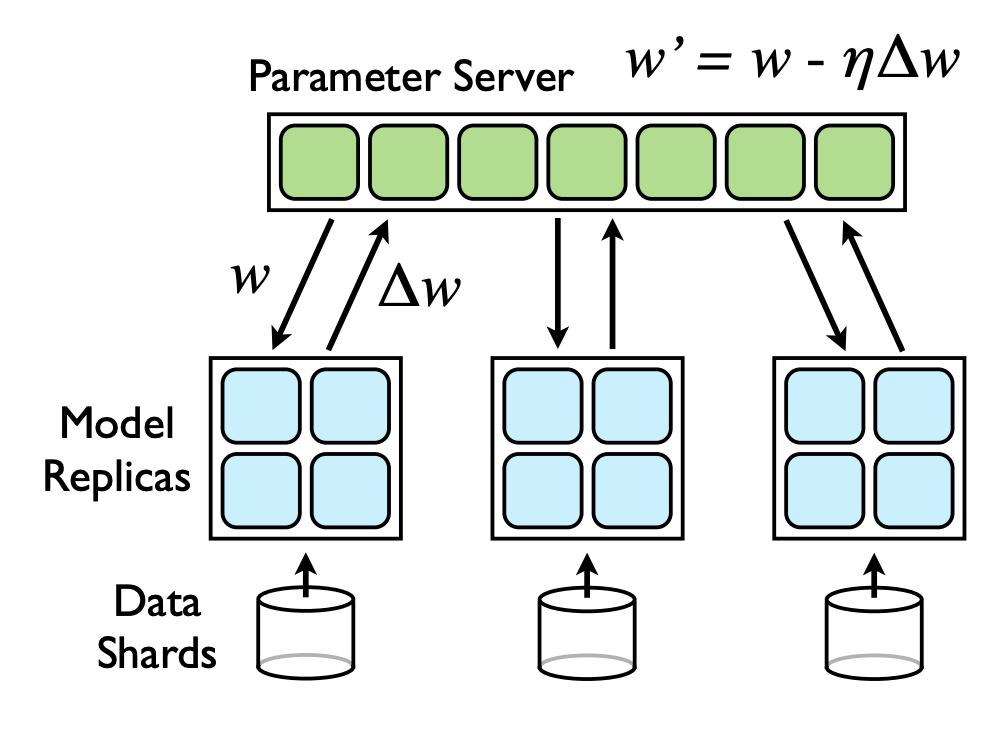
\includegraphics[width=0.7\linewidth]{figures/algos/sgd.png}
    \caption{Async-SGD: Model replicas asynchronously fetch parameters w and push gradients \(\Delta w\) to the parameter server.}
    \label{fig:sgd}
\end{figure}

\clearpage

Since then a couple of different RL algorithms have proposed including:

$\bullet$ \textit{A distributed version of Deep Q-Networks}~\parencite{ong2015distributed} where they adapt the \textit{DistBelief} software framework to the context of efficiently
training reinforcement learning agents to distribute the deep Q-network training. resulting the method is completely asynchronous and scales well with the number of machines. 

$\bullet$ \textit{Massively parallel methods for DRL}~\ref{fig:gorila} \textbf{(Gorilla)}~\parencite{nair2015massively}, which uses a distributed experience replay buffer (and no prioritization). This architecture~\ref{fig:gorila_arch} uses four main components: \textit{parallel actors} that generate new behaviour, \textit{parallel learners} that are trained from stored experience, \textit{a distributed neural network} to represent the value function or behaviour policy, and \textit{a distributed store of experience} with no prioritization. It was applied to \textbf{49 games} from Atari 2600 games from the Arcade Learning Environment, using identical hyperparameters. The performance~\ref{fig:gorila_results} surpassed \textit{non-distributed DQN} in \textbf{41} of the 49 games and also reduced the wall-time required to achieve these results by an order of magnitude on most games.

\begin{figure}[H]
	\centering
	\begin{subfigure}[b]{0.4\textwidth}
		\centering
		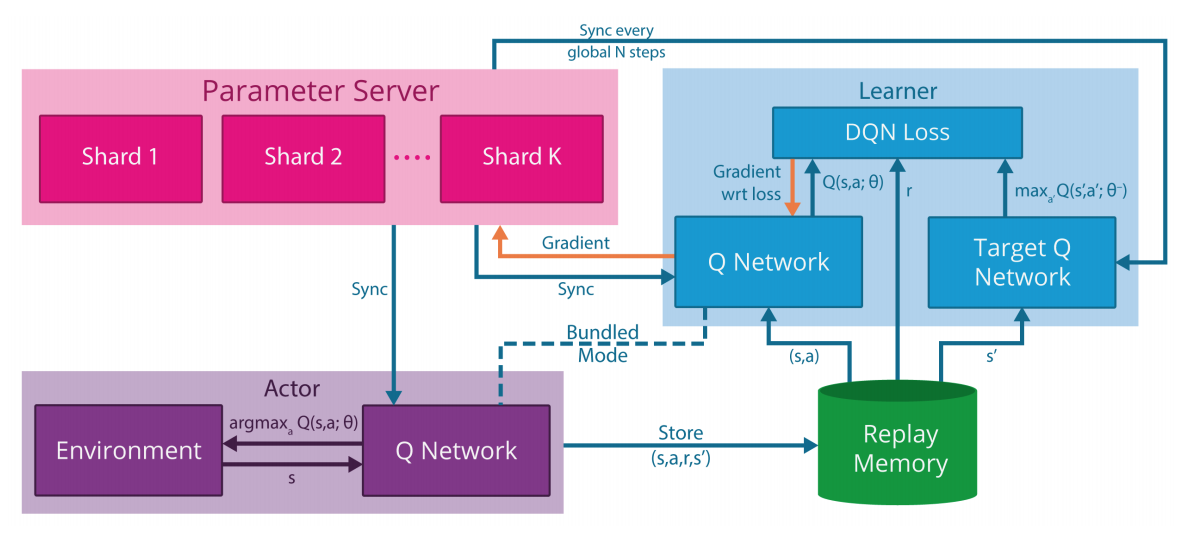
\includegraphics[width=\textwidth]{figures/algos/gorila.png}
		\caption{Agent parallelises the training procedure by separating out learners, actors and parameter server}
		\label{fig:gorila_arch}
    \end{subfigure}
    \hfill
	\begin{subfigure}[b]{0.4\textwidth}
		\centering
		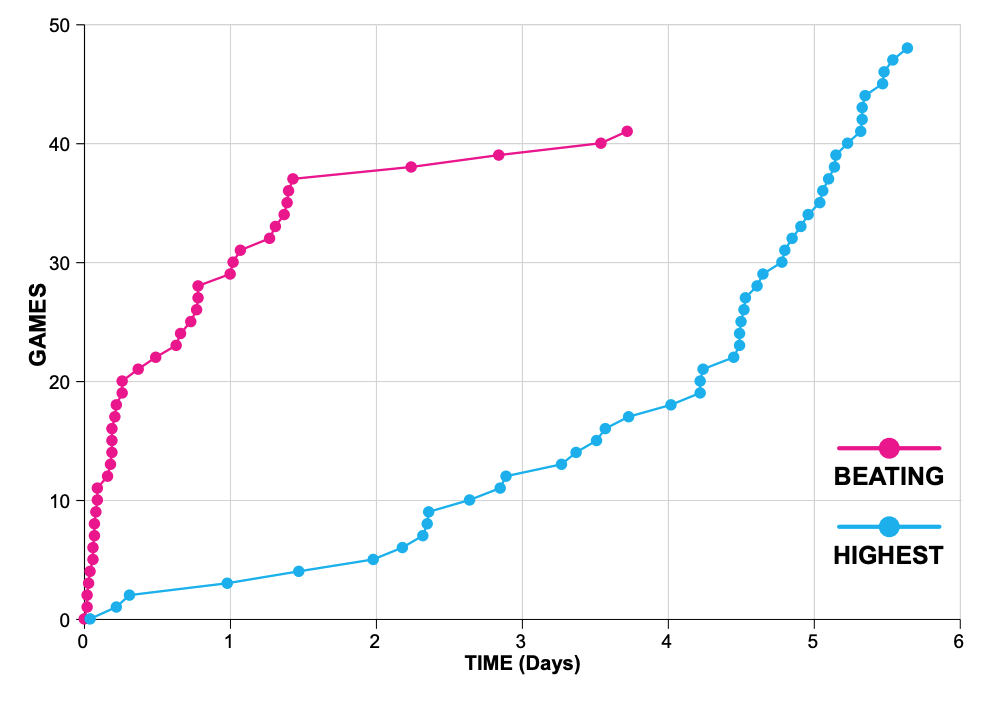
\includegraphics[width=\textwidth]{figures/algos/gorila_results.png}
        \caption{Red curve: time to surpass single DQN\\
                Blue curve: time to reach its peak performance}
		\label{fig:gorila_results}
	\end{subfigure}
	\hfill
	   \caption{The Gorila Architecture \& Results}
	   \label{fig:gorila}
\end{figure}

$\bullet$ \textit{Asynchronous methods for DRL}~\ref{fig:a3c} \textbf{(A3C)}~\parencite{mnih2016asynchronous}, in which they present asynchronous variants of four standard reinforcement learning algorithms and show that parallel actor-learners have a stabilizing effect on training allowing all four methods to successfully train neural network controllers using asynchronous gradient descent for optimization. The algorithms~\ref{fig:a3c_workflow} used multiple threads to run copies of the environment and generate uncorrelated sequences of training samples. Parameters were then sent to a shared parameter server at regular intervals. Because this promotes non-stationarity for the sequences of SARSA tuples, experience replay is not necessarily needed. The implementations of RMSProp and Momentum SGD used by the authors employed a Hogwild-inpsired~\parencite{recht2011hogwild} lock free scheme for maximum efficiency. A3C is the ``best'' agent that was presented in this paper. It is an asynchronous advantage actor-critic algorithm. It maintains an approximation of the policy, an estimate of the value function, and computes an ``advantage'' function and a variance-reducing baseline~\parencite{degris2012off}. An entropy regularization term was also used to discourage premature convergence. The A3C performance overpassed gorila and add some enhancement including faster updates, removing  the replay buffer, and moving to Actor-Critic (from Q learning).

The State-of-the-art results~\ref{fig:a3c_results} were obtained on some of the Atari games (ALE). An LSTM-based A3C agent was tested with Deepmind’s Labyrinth environment. They also tested on the TORCS car racing environment and MuJoCo, the continuous-space physics simulation engine.

\begin{figure}[H]
	\centering
	\begin{subfigure}[b]{0.3\textwidth}
		\centering
		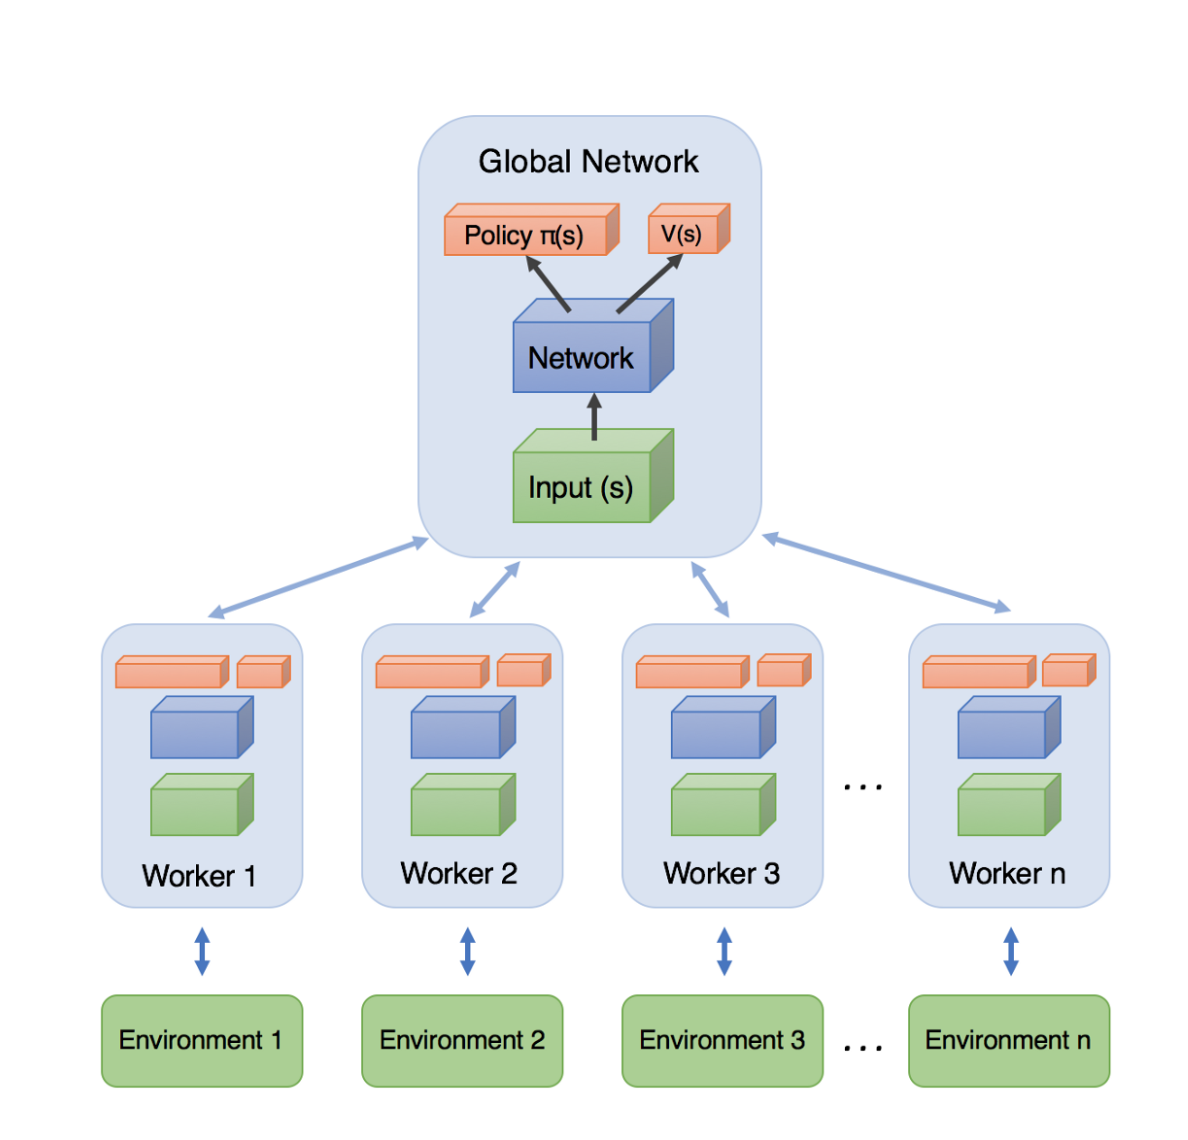
\includegraphics[width=\textwidth]{figures/algos/a3c.png}
		\caption{A3C high-level architecture.}
		\label{fig:a3c_arch}
    \end{subfigure}
    \hfill
    \begin{subfigure}[b]{0.3\textwidth}
		\centering
		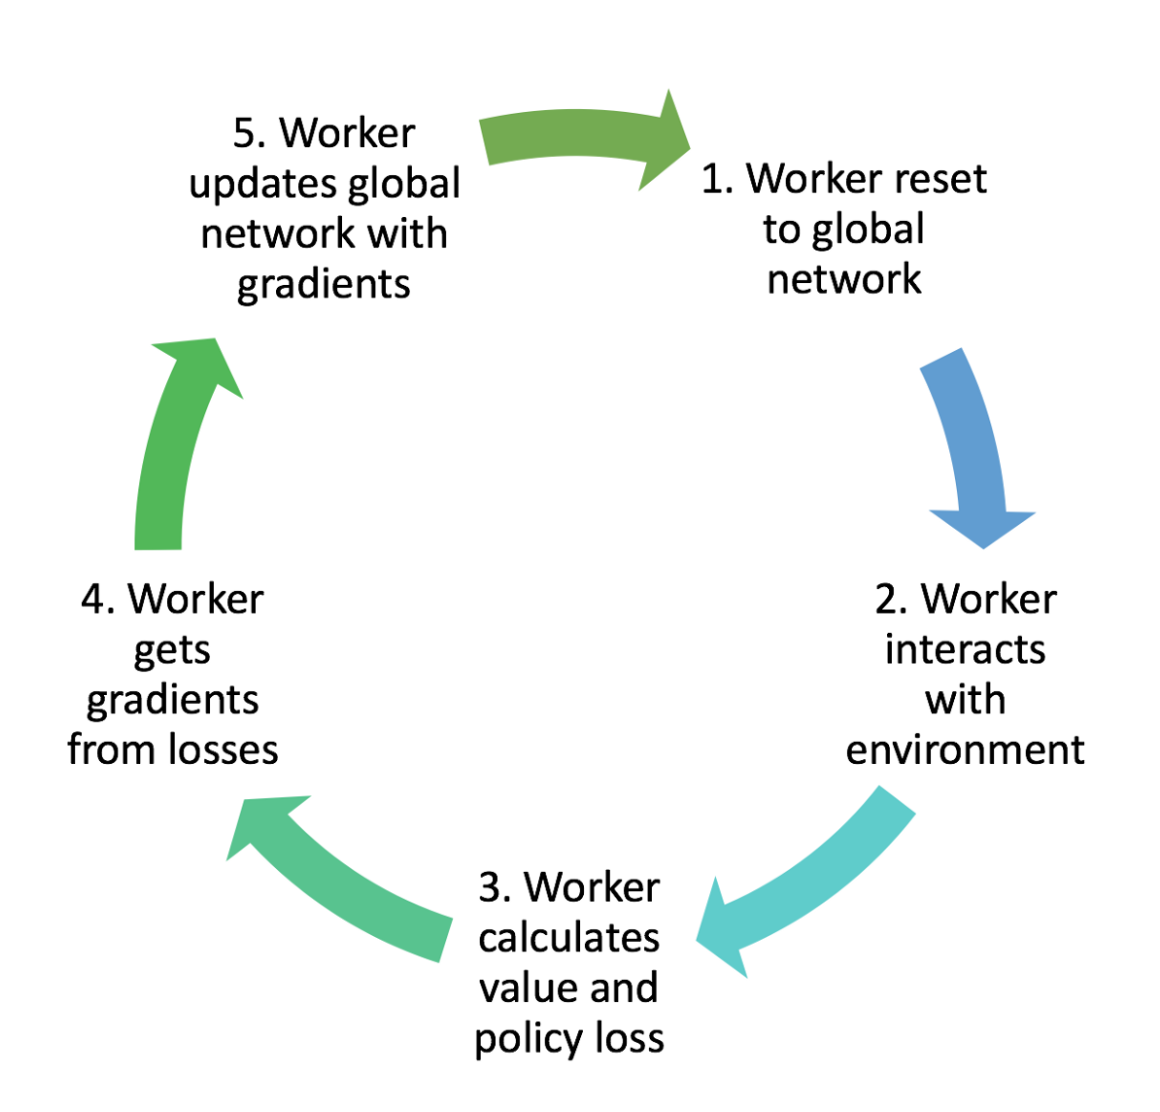
\includegraphics[width=\textwidth]{figures/algos/a3c_workflow.png}
		\caption{Training workflow of each worker agent in A3C.}
		\label{fig:a3c_workflow}
    \end{subfigure}
    \hfill
	\begin{subfigure}[b]{0.3\textwidth}
		\centering
		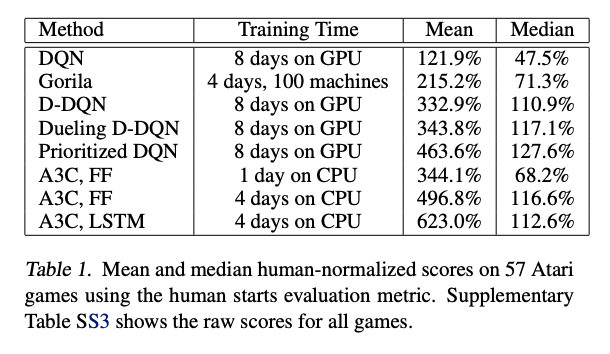
\includegraphics[width=\textwidth]{figures/algos/a3c_results.png}
        \caption{A3C Results}
		\label{fig:a3c_results}
	\end{subfigure}
	\hfill
	   \caption{The A3C Architecture, workflow \& Results}
	   \label{fig:a3c}
\end{figure}

Another direction with some alternatives to \textit{asynchronous SGD} methods which includes distributed BA3C~\parencite{adamski2018distributed}, Evolution strategies~\parencite{salimans2017evolution} using evolutionary processes and 

$\bullet$ \textit{Distributed Prioritized Experience Replay}~\ref{fig:apex} \textbf{(Ape-X)}~\parencite{horgan2018distributed} which use a distributed replay with a synchronous learner. They focused on on applying the Ape-X framework to DQN and DPG, also it could  be combined with any other off-policy reinforcement learning update. 

The main idea of this paper is to scale up the experience replay data by having many actors running in parallel  collect samples of experience. The actors periodically pool their samples into a centralized data repository, which is used for experience replay for a centralized learner to select from it in a prioritized fashion~\parencite{schaul2015prioritized} and update neural network parameters. Those parameters then get copied back to the actors. Hence, they step over and complement standard distributed training approaches~\parencite{dean2012large} of neural networks which focus on parallelizing the computation of gradients to \textit{distribute the generation and selection of experience data}, which suffices to improve results.

This architecture achieved state of the art results~\ref{fig:apex_results} in a wide range of discrete and continuous tasks, both in terms of wall-clock learning speed and final performance

\begin{figure}[H]
	\centering
	\begin{subfigure}[b]{0.4\textwidth}
		\centering
		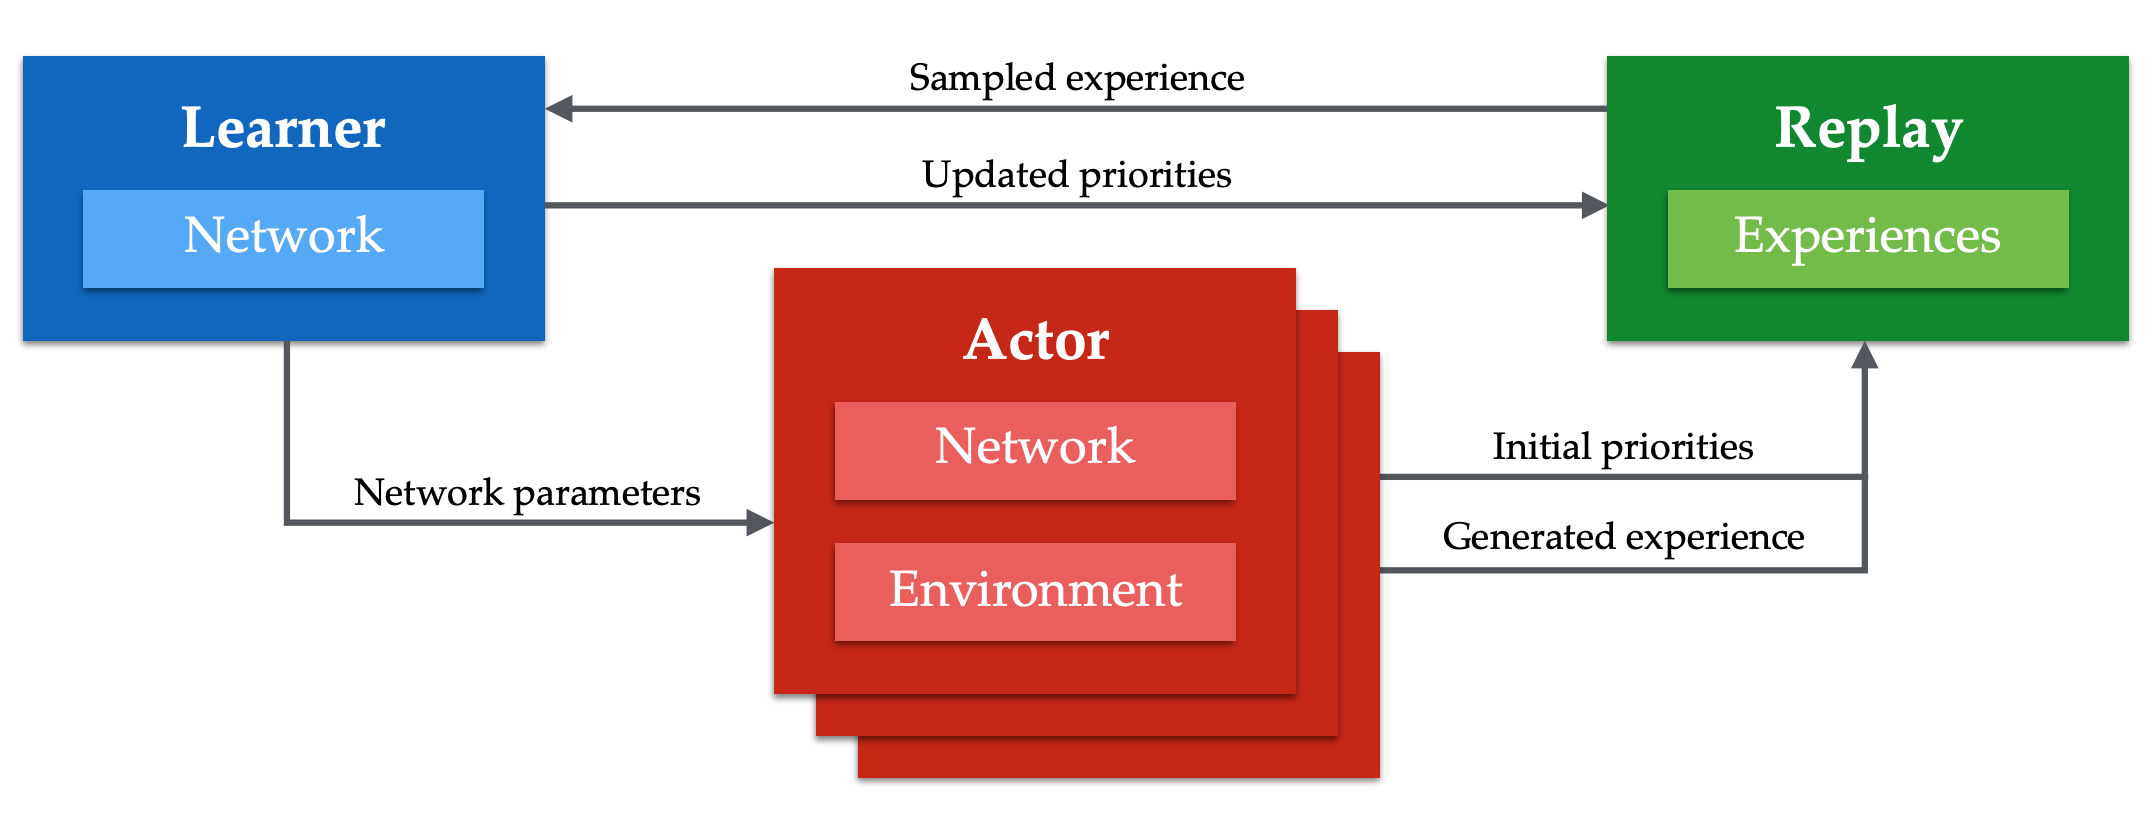
\includegraphics[width=\textwidth]{figures/algos/apex.png}
		\caption{The Ape-X architecture}
		\label{fig:apex_arch}
    \end{subfigure}
    \hfill
	\begin{subfigure}[b]{0.4\textwidth}
		\centering
		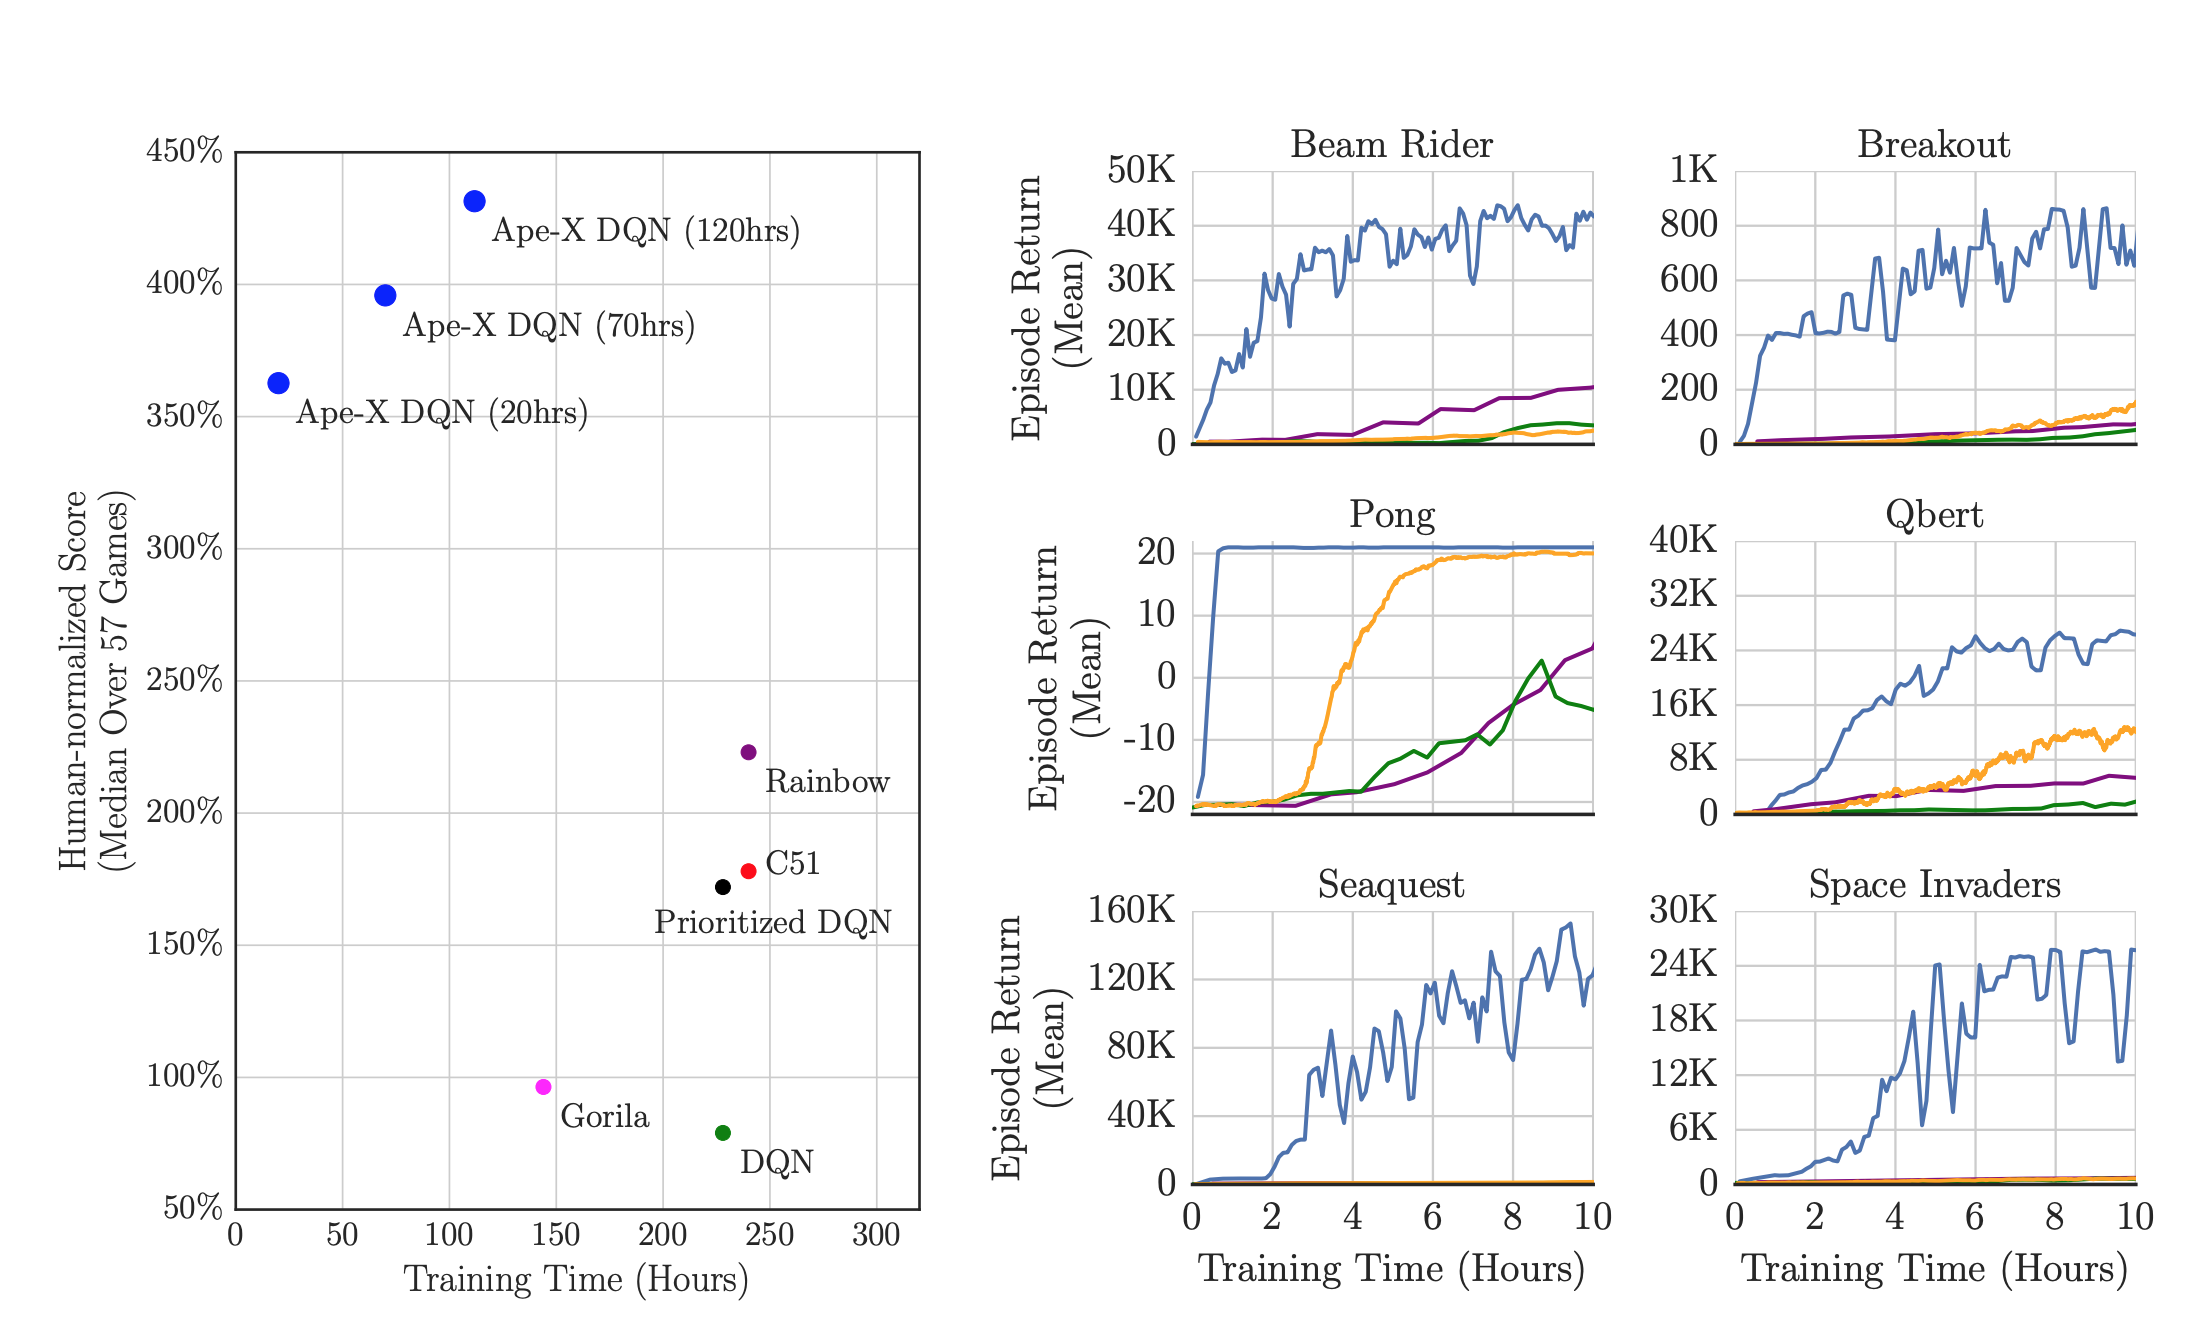
\includegraphics[width=\textwidth]{figures/algos/apex_results.png}
        \caption{Ape-X Performance compared with other RL algorithms}
		\label{fig:apex_results}
	\end{subfigure}
	\hfill
	   \caption{The Ape-X Architecture \& Results}
	   \label{fig:apex}
\end{figure}

Other research have attempt to scale up by using multiple GPUs and utilizing them. The simplest method is batched A2C~\parencite{clemente2017efficient} in which with every step produces a batch of actions and applies them to a batch of environments. BA3C~\parencite{babaeizadeh2016ga3c} another method which uses asynchronous data collection to effectively utilize GPUs.

The state of the art method in distributed reinforcement learning is \textbf{Impala}~\parencite{espeholt2018impala}, which is able to do \textbf{30 different challenging tasks} that require various aspects of \textit{learning, memory, and navigation}. This method of learning has already been used for some amazing achievements such as endowing an AI with emotions and learning complex games like ``Go'' and ``Poker''.


\section{Research Statement}
In this project we experiment the effect of training different environment in both non-distributed and distribute training modes. We compare between the state of the art algorithms in the field and effect of distributing them and using parallel environment while training the agents.

\section{Overview and Outline}
The work is organized as follows. In \autoref{chapter:Background and Foundations}, the theoretical background linked to reinforcement learning and the Markov decision process framework are introduced. Furthermore, we discuss the use of deep learning in RL framework and the state of the art algorithms, we also discuss the challenging problems associated with reinforcement learning.  The \autoref{chapter:Background and Foundations} presents the experiment setting used in \autoref{chapter:Background and Foundations}. The latter presents, examines and discusses the results. Finally, \autoref{chapter:Background and Foundations} discusses future work and concludes.